\section{ISISDLM::Keyword\-Handler Class Reference}
\label{classISISDLM_1_1KeywordHandler}\index{ISISDLM::KeywordHandler@{ISISDLM::KeywordHandler}}
{\tt \#include $<$Keyword\-Handler.h$>$}

\subsection*{Public Types}
\begin{CompactItemize}
\item 
typedef TNT::Array1D$<$ short int $>$ {\bf Occurance}
\item 
enum {\bf Key\-Type} \{ {\bf String}, 
{\bf Double}, 
{\bf Integer}
 \}
\item 
enum {\bf Aggregate\-Type} \{ {\bf None}, 
{\bf Keyword}, 
{\bf Group}, 
{\bf Object}
 \}
\end{CompactItemize}
\subsection*{Public Member Functions}
\begin{CompactItemize}
\item 
{\bf Keyword\-Handler} ()
\item 
{\bf Keyword\-Handler} (const std::string \&kspec, const {\bf Occurance} $\ast$occurs=0)
\item 
virtual {\bf $\sim$Keyword\-Handler} ()
\item 
void {\bf set\-Keyword\-Spec} (const std::string \&kspec, const {\bf Occurance} $\ast$occurs=0)
\item 
bool {\bf Exists} (Isis::Pvl \&pvl, int \&nvals)
\item 
int {\bf size} (Isis::Pvl \&pvl)
\item 
std::string {\bf Unit} (Isis::Pvl \&pvl, int nth=0)
\item 
template$<$class T$>$ bool {\bf Fetch} (Isis::Pvl \&pvl, TNT::Array1D$<$ T $>$ \&vals)
\item 
template$<$class T$>$ bool {\bf Fetch} (Isis::Pvl \&pvl, T \&val, int nth=0)
\item 
void {\bf Create} (const std::string \&name, {\bf Aggregate\-Type} ktype=Group)
\item 
template$<$class T$>$ void {\bf Put} (Isis::Pvl \&pvl, const TNT::Array1D$<$ T $>$ \&vals, const std::string \&unit=\char`\"{}\char`\"{})
\item 
template$<$class T$>$ void {\bf Put} (Isis::Pvl \&pvl, T \&val, int nth=0)
\item 
bool {\bf Delete} (Isis::Pvl \&pvl)
\end{CompactItemize}
\subsection*{Static Public Attributes}
\begin{CompactItemize}
\item 
const char $\ast$const {\bf ID} = \char`\"{}\$Revision: 1.2 \$ \$Date: 2004/11/02 15:38:53 \$\char`\"{}
\begin{CompactList}\small\item\em Class version. \item\end{CompactList}\end{CompactItemize}
\subsection*{Private Types}
\begin{CompactItemize}
\item 
typedef std::vector$<$ {\bf Key\-Spec} $>$ {\bf Pvl\-Spec\-List}
\item 
typedef Pvl\-Spec\-List::const\_\-iterator {\bf Pvl\-Spec\-List\-Const\-Iter}
\item 
typedef std::vector$<$ {\bf Pvl\-Aggregate} $>$ {\bf Aggregate\-List}
\end{CompactItemize}
\subsection*{Private Member Functions}
\begin{CompactItemize}
\item 
void {\bf parse\-Spec} (const std::string \&kspec, const {\bf Occurance} $\ast$occurs=0)
\item 
{\bf Occurance} {\bf get\-Occurance} (int n, const {\bf Occurance} \&occurs) const
\item 
int {\bf resolve} (Isis::Pvl \&pvl, const {\bf Pvl\-Spec\-List} \&specs, {\bf Aggregate\-List} \&elements)
\item 
int {\bf resolve\-Object} (Isis::Pvl\-Object $\ast$obj, {\bf Pvl\-Spec\-List\-Const\-Iter} \&current, {\bf Pvl\-Spec\-List\-Const\-Iter} \&end, {\bf Aggregate\-List} \&elements)
\item 
int {\bf resolve\-Group} (Isis::Pvl\-Object $\ast$obj, {\bf Pvl\-Spec\-List\-Const\-Iter} \&current, {\bf Pvl\-Spec\-List\-Const\-Iter} \&end, {\bf Aggregate\-List} \&elements)
\item 
int {\bf resolve\-Keyword} (Isis::Pvl\-Container $\ast$pvl, {\bf Pvl\-Spec\-List\-Const\-Iter} \&current, {\bf Pvl\-Spec\-List\-Const\-Iter} \&end, {\bf Aggregate\-List} \&elements)
\end{CompactItemize}
\subsection*{Private Attributes}
\begin{CompactItemize}
\item 
{\bf Pvl\-Spec\-List} {\bf \_\-kspec}
\end{CompactItemize}


\subsection{Detailed Description}
Specification ISIS/PVL keyword support The {\em {\bf Keyword\-Handler}\/} class handles keyword manipulation for DLM activities. 



\subsection{Member Typedef Documentation}
\index{ISISDLM::KeywordHandler@{ISISDLM::Keyword\-Handler}!AggregateList@{AggregateList}}
\index{AggregateList@{AggregateList}!ISISDLM::KeywordHandler@{ISISDLM::Keyword\-Handler}}
\subsubsection{\setlength{\rightskip}{0pt plus 5cm}typedef std::vector$<${\bf Pvl\-Aggregate}$>$ {\bf ISISDLM::Keyword\-Handler::Aggregate\-List}\hspace{0.3cm}{\tt  [private]}}\label{classISISDLM_1_1KeywordHandler_y2}


\index{ISISDLM::KeywordHandler@{ISISDLM::Keyword\-Handler}!Occurance@{Occurance}}
\index{Occurance@{Occurance}!ISISDLM::KeywordHandler@{ISISDLM::Keyword\-Handler}}
\subsubsection{\setlength{\rightskip}{0pt plus 5cm}typedef TNT::Array1D$<$short int$>$ {\bf ISISDLM::Keyword\-Handler::Occurance}}\label{classISISDLM_1_1KeywordHandler_w0}


\index{ISISDLM::KeywordHandler@{ISISDLM::Keyword\-Handler}!PvlSpecList@{PvlSpecList}}
\index{PvlSpecList@{PvlSpecList}!ISISDLM::KeywordHandler@{ISISDLM::Keyword\-Handler}}
\subsubsection{\setlength{\rightskip}{0pt plus 5cm}typedef std::vector$<${\bf Key\-Spec}$>$ {\bf ISISDLM::Keyword\-Handler::Pvl\-Spec\-List}\hspace{0.3cm}{\tt  [private]}}\label{classISISDLM_1_1KeywordHandler_y0}


\index{ISISDLM::KeywordHandler@{ISISDLM::Keyword\-Handler}!PvlSpecListConstIter@{PvlSpecListConstIter}}
\index{PvlSpecListConstIter@{PvlSpecListConstIter}!ISISDLM::KeywordHandler@{ISISDLM::Keyword\-Handler}}
\subsubsection{\setlength{\rightskip}{0pt plus 5cm}typedef Pvl\-Spec\-List::const\_\-iterator {\bf ISISDLM::Keyword\-Handler::Pvl\-Spec\-List\-Const\-Iter}\hspace{0.3cm}{\tt  [private]}}\label{classISISDLM_1_1KeywordHandler_y1}




\subsection{Member Enumeration Documentation}
\index{ISISDLM::KeywordHandler@{ISISDLM::Keyword\-Handler}!AggregateType@{AggregateType}}
\index{AggregateType@{AggregateType}!ISISDLM::KeywordHandler@{ISISDLM::Keyword\-Handler}}
\subsubsection{\setlength{\rightskip}{0pt plus 5cm}enum {\bf ISISDLM::Keyword\-Handler::Aggregate\-Type}}\label{classISISDLM_1_1KeywordHandler_w9}


\begin{Desc}
\item[Enumeration values: ]\par
\begin{description}
\index{None@{None}!ISISDLM::KeywordHandler@{ISISDLM::KeywordHandler}}\index{ISISDLM::KeywordHandler@{ISISDLM::KeywordHandler}!None@{None}}\item[{\em 
{\em None}\label{classISISDLM_1_1KeywordHandler_w9w4}
}]\index{Keyword@{Keyword}!ISISDLM::KeywordHandler@{ISISDLM::KeywordHandler}}\index{ISISDLM::KeywordHandler@{ISISDLM::KeywordHandler}!Keyword@{Keyword}}\item[{\em 
{\em Keyword}\label{classISISDLM_1_1KeywordHandler_w9w5}
}]\index{Group@{Group}!ISISDLM::KeywordHandler@{ISISDLM::KeywordHandler}}\index{ISISDLM::KeywordHandler@{ISISDLM::KeywordHandler}!Group@{Group}}\item[{\em 
{\em Group}\label{classISISDLM_1_1KeywordHandler_w9w6}
}]\index{Object@{Object}!ISISDLM::KeywordHandler@{ISISDLM::KeywordHandler}}\index{ISISDLM::KeywordHandler@{ISISDLM::KeywordHandler}!Object@{Object}}\item[{\em 
{\em Object}\label{classISISDLM_1_1KeywordHandler_w9w7}
}]\end{description}
\end{Desc}

\index{ISISDLM::KeywordHandler@{ISISDLM::Keyword\-Handler}!KeyType@{KeyType}}
\index{KeyType@{KeyType}!ISISDLM::KeywordHandler@{ISISDLM::Keyword\-Handler}}
\subsubsection{\setlength{\rightskip}{0pt plus 5cm}enum {\bf ISISDLM::Keyword\-Handler::Key\-Type}}\label{classISISDLM_1_1KeywordHandler_w8}


\begin{Desc}
\item[Enumeration values: ]\par
\begin{description}
\index{String@{String}!ISISDLM::KeywordHandler@{ISISDLM::KeywordHandler}}\index{ISISDLM::KeywordHandler@{ISISDLM::KeywordHandler}!String@{String}}\item[{\em 
{\em String}\label{classISISDLM_1_1KeywordHandler_w8w1}
}]\index{Double@{Double}!ISISDLM::KeywordHandler@{ISISDLM::KeywordHandler}}\index{ISISDLM::KeywordHandler@{ISISDLM::KeywordHandler}!Double@{Double}}\item[{\em 
{\em Double}\label{classISISDLM_1_1KeywordHandler_w8w2}
}]\index{Integer@{Integer}!ISISDLM::KeywordHandler@{ISISDLM::KeywordHandler}}\index{ISISDLM::KeywordHandler@{ISISDLM::KeywordHandler}!Integer@{Integer}}\item[{\em 
{\em Integer}\label{classISISDLM_1_1KeywordHandler_w8w3}
}]\end{description}
\end{Desc}



\subsection{Constructor \& Destructor Documentation}
\index{ISISDLM::KeywordHandler@{ISISDLM::Keyword\-Handler}!KeywordHandler@{KeywordHandler}}
\index{KeywordHandler@{KeywordHandler}!ISISDLM::KeywordHandler@{ISISDLM::Keyword\-Handler}}
\subsubsection{\setlength{\rightskip}{0pt plus 5cm}ISISDLM::Keyword\-Handler::Keyword\-Handler ()\hspace{0.3cm}{\tt  [inline]}}\label{classISISDLM_1_1KeywordHandler_a0}


\index{ISISDLM::KeywordHandler@{ISISDLM::Keyword\-Handler}!KeywordHandler@{KeywordHandler}}
\index{KeywordHandler@{KeywordHandler}!ISISDLM::KeywordHandler@{ISISDLM::Keyword\-Handler}}
\subsubsection{\setlength{\rightskip}{0pt plus 5cm}ISISDLM::Keyword\-Handler::Keyword\-Handler (const std::string \& {\em kspec}, const {\bf Occurance} $\ast$ {\em occurs} = 0)}\label{classISISDLM_1_1KeywordHandler_a1}




Here is the call graph for this function:\begin{figure}[H]
\begin{center}
\leavevmode
\includegraphics[width=389pt]{classISISDLM_1_1KeywordHandler_a1_cgraph}
\end{center}
\end{figure}
\index{ISISDLM::KeywordHandler@{ISISDLM::Keyword\-Handler}!~KeywordHandler@{$\sim$KeywordHandler}}
\index{~KeywordHandler@{$\sim$KeywordHandler}!ISISDLM::KeywordHandler@{ISISDLM::Keyword\-Handler}}
\subsubsection{\setlength{\rightskip}{0pt plus 5cm}virtual ISISDLM::Keyword\-Handler::$\sim${\bf Keyword\-Handler} ()\hspace{0.3cm}{\tt  [inline, virtual]}}\label{classISISDLM_1_1KeywordHandler_a2}




\subsection{Member Function Documentation}
\index{ISISDLM::KeywordHandler@{ISISDLM::Keyword\-Handler}!Create@{Create}}
\index{Create@{Create}!ISISDLM::KeywordHandler@{ISISDLM::Keyword\-Handler}}
\subsubsection{\setlength{\rightskip}{0pt plus 5cm}void ISISDLM::Keyword\-Handler::Create (const std::string \& {\em name}, {\bf Aggregate\-Type} {\em ktype} = Group)}\label{classISISDLM_1_1KeywordHandler_a9}


\index{ISISDLM::KeywordHandler@{ISISDLM::Keyword\-Handler}!Delete@{Delete}}
\index{Delete@{Delete}!ISISDLM::KeywordHandler@{ISISDLM::Keyword\-Handler}}
\subsubsection{\setlength{\rightskip}{0pt plus 5cm}bool ISISDLM::Keyword\-Handler::Delete (Isis::Pvl \& {\em pvl})}\label{classISISDLM_1_1KeywordHandler_a12}


\index{ISISDLM::KeywordHandler@{ISISDLM::Keyword\-Handler}!Exists@{Exists}}
\index{Exists@{Exists}!ISISDLM::KeywordHandler@{ISISDLM::Keyword\-Handler}}
\subsubsection{\setlength{\rightskip}{0pt plus 5cm}bool ISISDLM::Keyword\-Handler::Exists (Isis::Pvl \& {\em pvl}, int \& {\em nvals})}\label{classISISDLM_1_1KeywordHandler_a4}




Here is the call graph for this function:\begin{figure}[H]
\begin{center}
\leavevmode
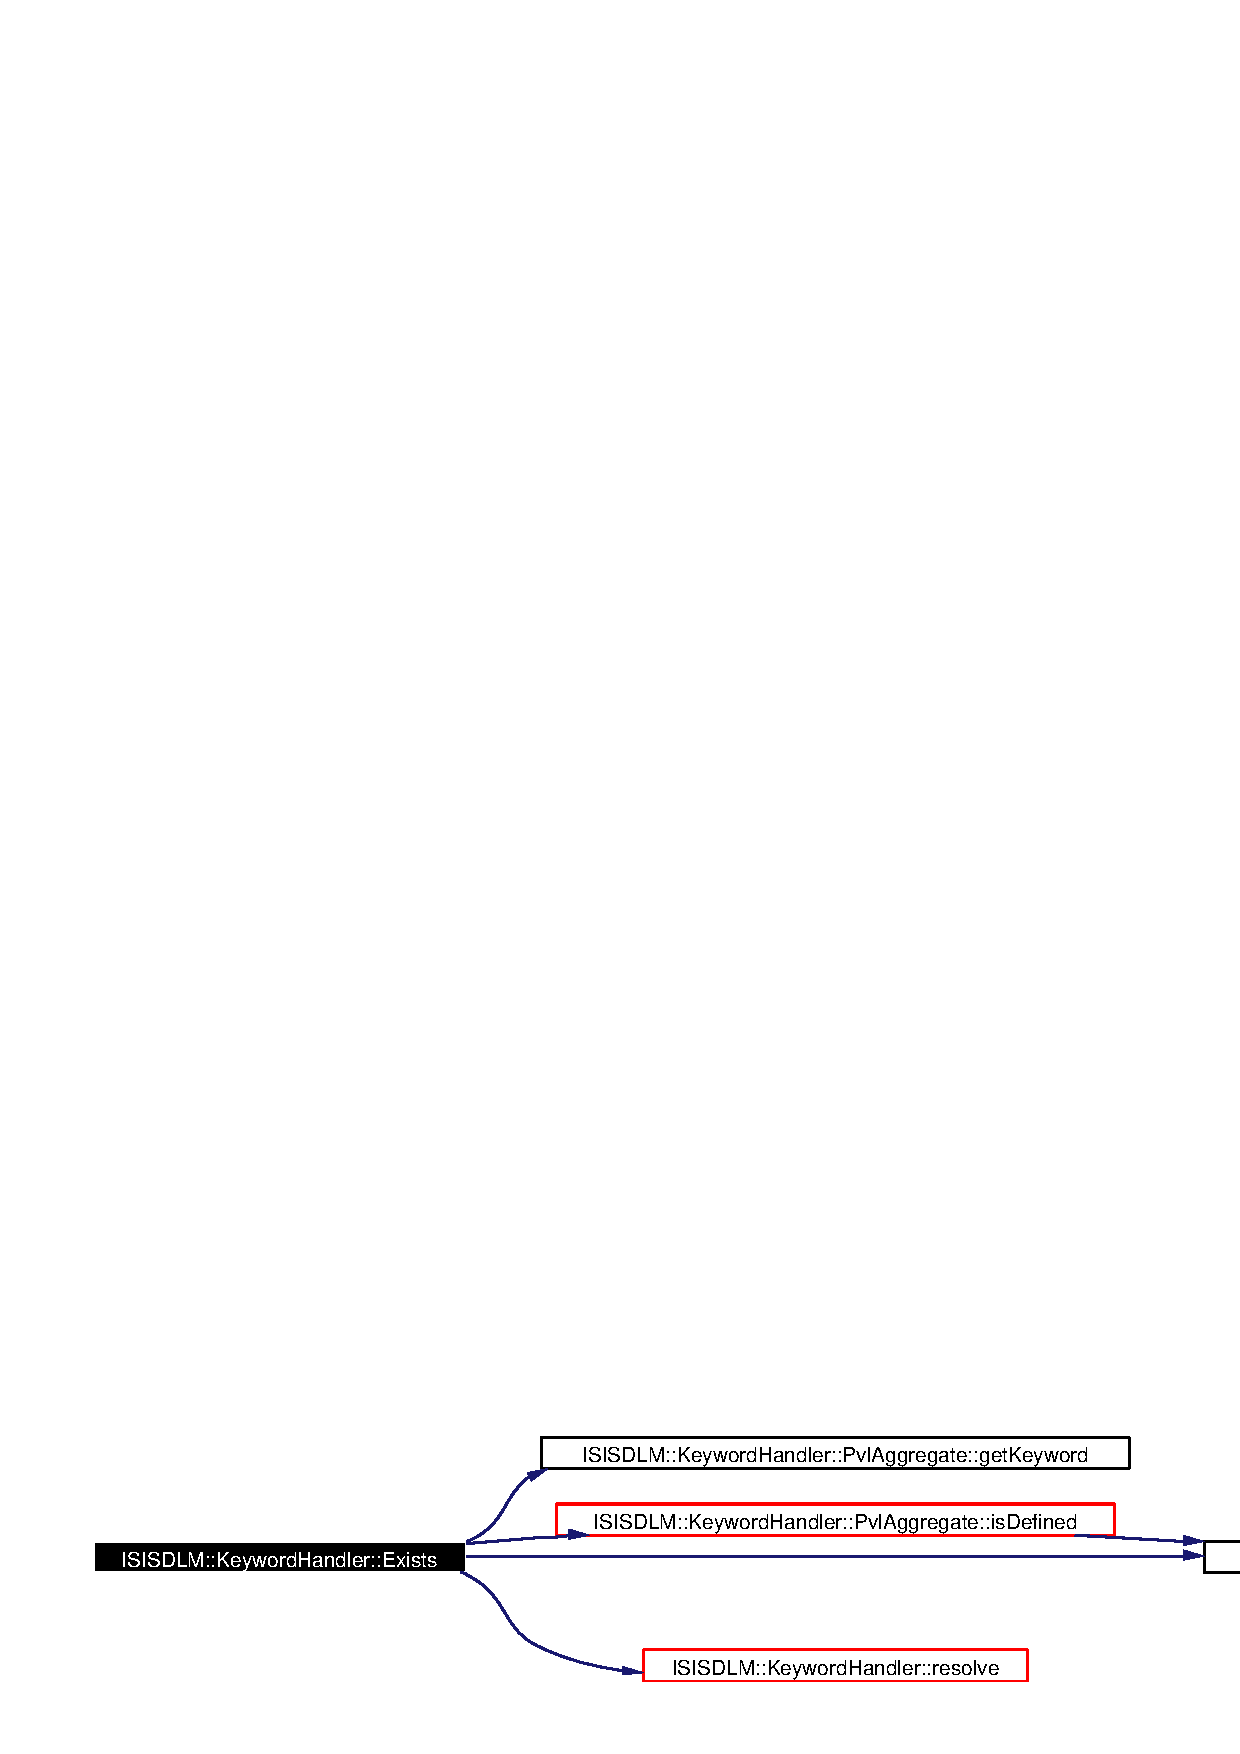
\includegraphics[width=420pt]{classISISDLM_1_1KeywordHandler_a4_cgraph}
\end{center}
\end{figure}
\index{ISISDLM::KeywordHandler@{ISISDLM::Keyword\-Handler}!Fetch@{Fetch}}
\index{Fetch@{Fetch}!ISISDLM::KeywordHandler@{ISISDLM::Keyword\-Handler}}
\subsubsection{\setlength{\rightskip}{0pt plus 5cm}template$<$class T$>$ bool ISISDLM::Keyword\-Handler::Fetch (Isis::Pvl \& {\em pvl}, T \& {\em val}, int {\em nth} = 0)}\label{classISISDLM_1_1KeywordHandler_a8}




Here is the call graph for this function:\begin{figure}[H]
\begin{center}
\leavevmode
\includegraphics[width=400pt]{classISISDLM_1_1KeywordHandler_a8_cgraph}
\end{center}
\end{figure}
\index{ISISDLM::KeywordHandler@{ISISDLM::Keyword\-Handler}!Fetch@{Fetch}}
\index{Fetch@{Fetch}!ISISDLM::KeywordHandler@{ISISDLM::Keyword\-Handler}}
\subsubsection{\setlength{\rightskip}{0pt plus 5cm}template$<$class T$>$ bool ISISDLM::Keyword\-Handler::Fetch (Isis::Pvl \& {\em pvl}, TNT::Array1D$<$ T $>$ \& {\em vals})}\label{classISISDLM_1_1KeywordHandler_a7}




Here is the call graph for this function:\begin{figure}[H]
\begin{center}
\leavevmode
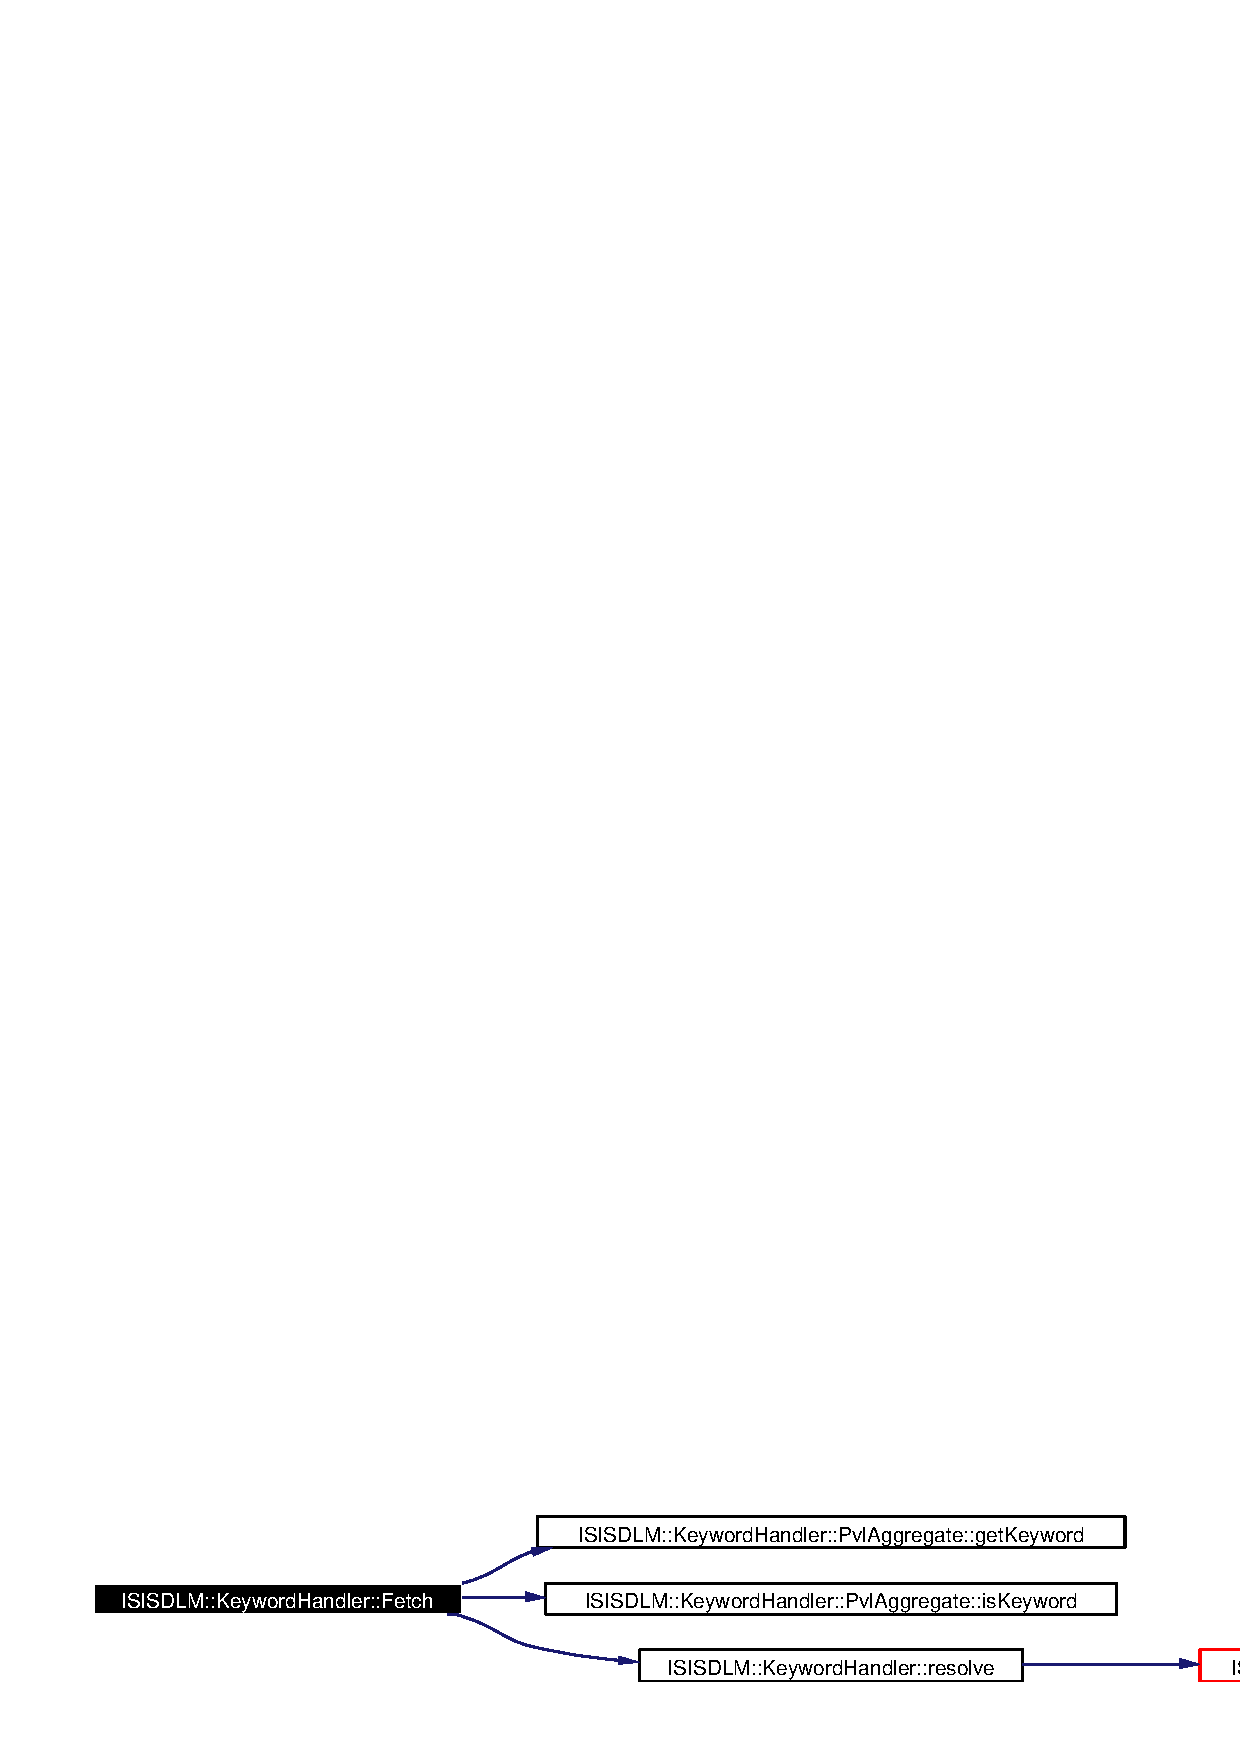
\includegraphics[width=400pt]{classISISDLM_1_1KeywordHandler_a7_cgraph}
\end{center}
\end{figure}
\index{ISISDLM::KeywordHandler@{ISISDLM::Keyword\-Handler}!getOccurance@{getOccurance}}
\index{getOccurance@{getOccurance}!ISISDLM::KeywordHandler@{ISISDLM::Keyword\-Handler}}
\subsubsection{\setlength{\rightskip}{0pt plus 5cm}{\bf Keyword\-Handler::Occurance} ISISDLM::Keyword\-Handler::get\-Occurance (int {\em n}, const {\bf Occurance} \& {\em occurs}) const\hspace{0.3cm}{\tt  [private]}}\label{classISISDLM_1_1KeywordHandler_d1}


\index{ISISDLM::KeywordHandler@{ISISDLM::Keyword\-Handler}!parseSpec@{parseSpec}}
\index{parseSpec@{parseSpec}!ISISDLM::KeywordHandler@{ISISDLM::Keyword\-Handler}}
\subsubsection{\setlength{\rightskip}{0pt plus 5cm}void ISISDLM::Keyword\-Handler::parse\-Spec (const std::string \& {\em kspec}, const {\bf Occurance} $\ast$ {\em occurs} = 0)\hspace{0.3cm}{\tt  [private]}}\label{classISISDLM_1_1KeywordHandler_d0}




Here is the call graph for this function:\begin{figure}[H]
\begin{center}
\leavevmode
\includegraphics[width=252pt]{classISISDLM_1_1KeywordHandler_d0_cgraph}
\end{center}
\end{figure}
\index{ISISDLM::KeywordHandler@{ISISDLM::Keyword\-Handler}!Put@{Put}}
\index{Put@{Put}!ISISDLM::KeywordHandler@{ISISDLM::Keyword\-Handler}}
\subsubsection{\setlength{\rightskip}{0pt plus 5cm}template$<$class T$>$ void ISISDLM::Keyword\-Handler::Put (Isis::Pvl \& {\em pvl}, T \& {\em val}, int {\em nth} = 0)}\label{classISISDLM_1_1KeywordHandler_a11}




Here is the call graph for this function:\begin{figure}[H]
\begin{center}
\leavevmode
\includegraphics[width=395pt]{classISISDLM_1_1KeywordHandler_a11_cgraph}
\end{center}
\end{figure}
\index{ISISDLM::KeywordHandler@{ISISDLM::Keyword\-Handler}!Put@{Put}}
\index{Put@{Put}!ISISDLM::KeywordHandler@{ISISDLM::Keyword\-Handler}}
\subsubsection{\setlength{\rightskip}{0pt plus 5cm}template$<$class T$>$ void ISISDLM::Keyword\-Handler::Put (Isis::Pvl \& {\em pvl}, const TNT::Array1D$<$ T $>$ \& {\em vals}, const std::string \& {\em unit} = \char`\"{}\char`\"{})}\label{classISISDLM_1_1KeywordHandler_a10}




Here is the call graph for this function:\begin{figure}[H]
\begin{center}
\leavevmode
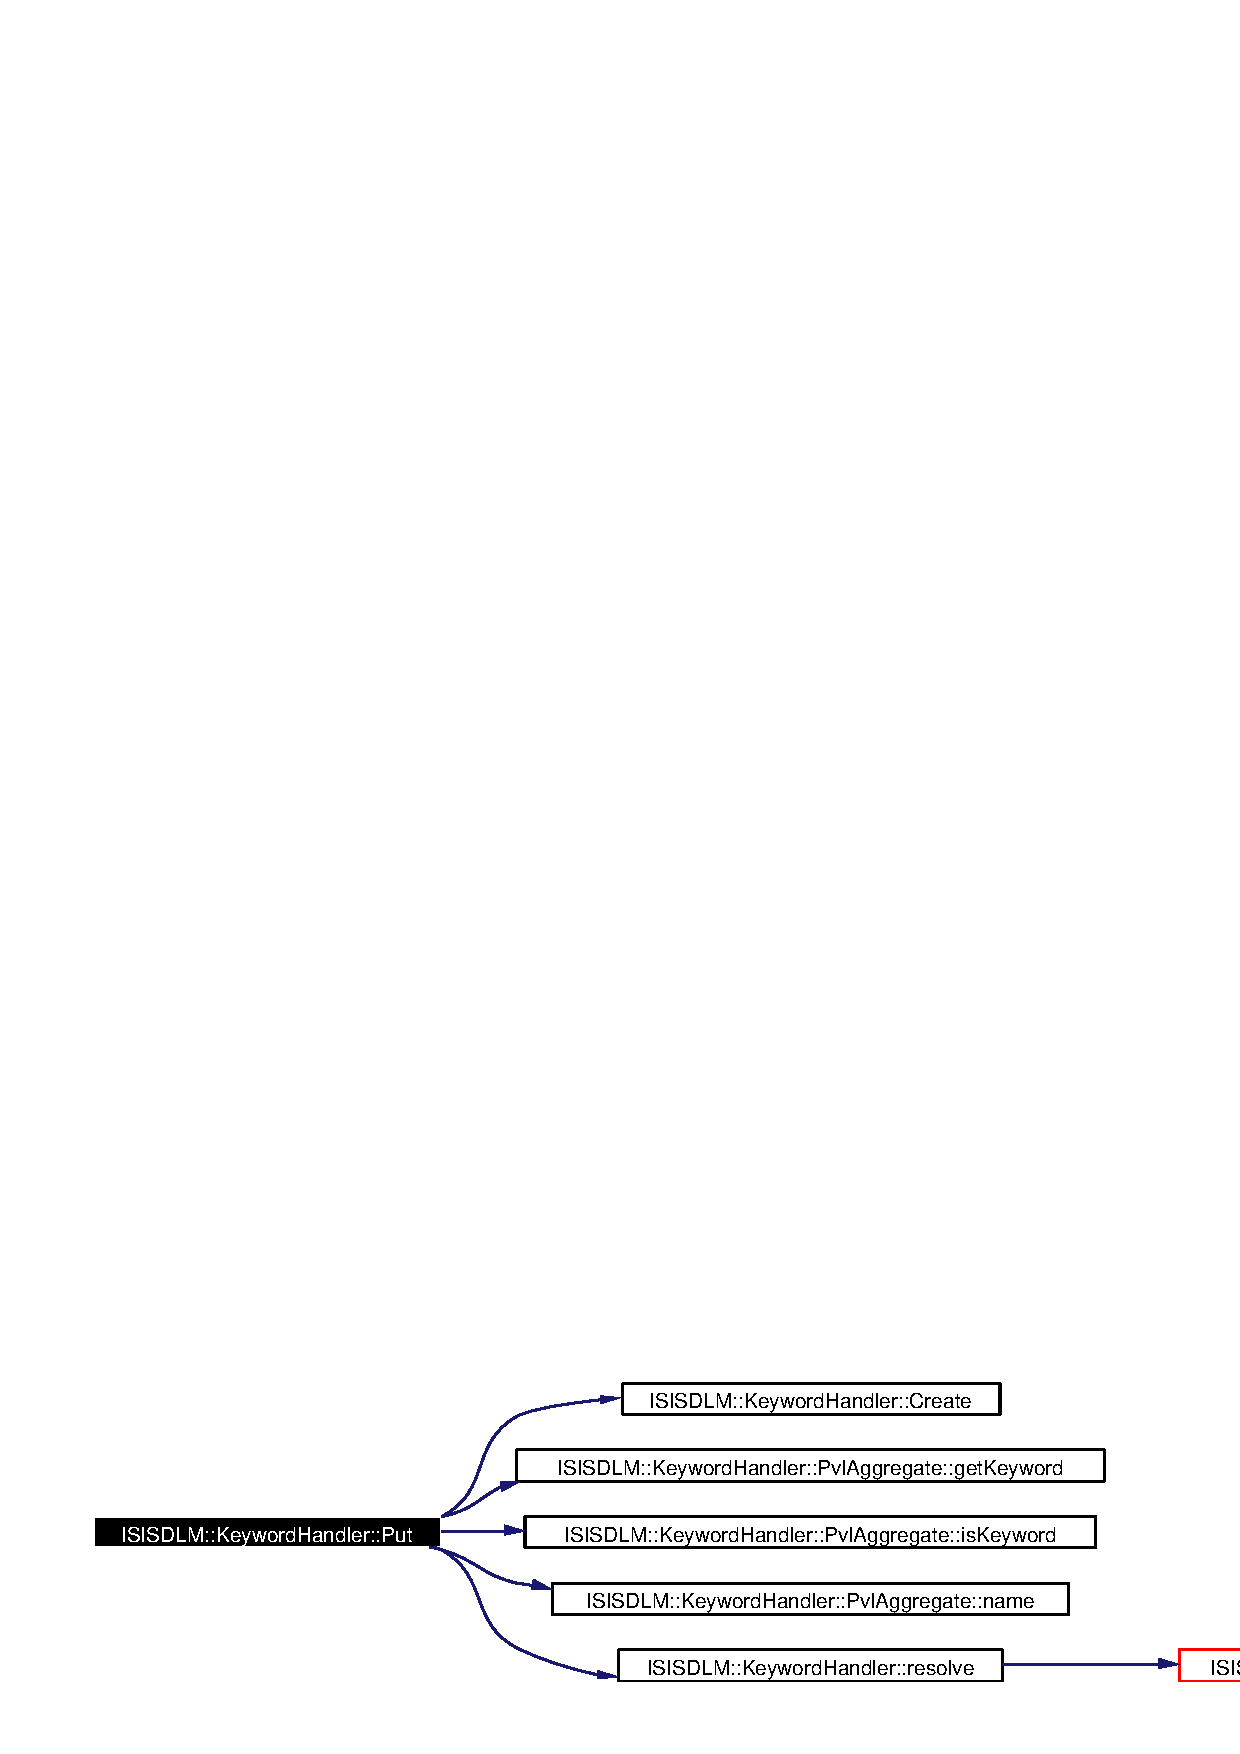
\includegraphics[width=395pt]{classISISDLM_1_1KeywordHandler_a10_cgraph}
\end{center}
\end{figure}
\index{ISISDLM::KeywordHandler@{ISISDLM::Keyword\-Handler}!resolve@{resolve}}
\index{resolve@{resolve}!ISISDLM::KeywordHandler@{ISISDLM::Keyword\-Handler}}
\subsubsection{\setlength{\rightskip}{0pt plus 5cm}int ISISDLM::Keyword\-Handler::resolve (Isis::Pvl \& {\em pvl}, const {\bf Pvl\-Spec\-List} \& {\em specs}, {\bf Aggregate\-List} \& {\em elements})\hspace{0.3cm}{\tt  [private]}}\label{classISISDLM_1_1KeywordHandler_d2}




Here is the call graph for this function:\begin{figure}[H]
\begin{center}
\leavevmode
\includegraphics[width=370pt]{classISISDLM_1_1KeywordHandler_d2_cgraph}
\end{center}
\end{figure}
\index{ISISDLM::KeywordHandler@{ISISDLM::Keyword\-Handler}!resolveGroup@{resolveGroup}}
\index{resolveGroup@{resolveGroup}!ISISDLM::KeywordHandler@{ISISDLM::Keyword\-Handler}}
\subsubsection{\setlength{\rightskip}{0pt plus 5cm}int ISISDLM::Keyword\-Handler::resolve\-Group (Isis::Pvl\-Object $\ast$ {\em obj}, {\bf Pvl\-Spec\-List\-Const\-Iter} \& {\em current}, {\bf Pvl\-Spec\-List\-Const\-Iter} \& {\em end}, {\bf Aggregate\-List} \& {\em elements})\hspace{0.3cm}{\tt  [private]}}\label{classISISDLM_1_1KeywordHandler_d4}




Here is the call graph for this function:\begin{figure}[H]
\begin{center}
\leavevmode
\includegraphics[width=268pt]{classISISDLM_1_1KeywordHandler_d4_cgraph}
\end{center}
\end{figure}
\index{ISISDLM::KeywordHandler@{ISISDLM::Keyword\-Handler}!resolveKeyword@{resolveKeyword}}
\index{resolveKeyword@{resolveKeyword}!ISISDLM::KeywordHandler@{ISISDLM::Keyword\-Handler}}
\subsubsection{\setlength{\rightskip}{0pt plus 5cm}int ISISDLM::Keyword\-Handler::resolve\-Keyword (Isis::Pvl\-Container $\ast$ {\em pvl}, {\bf Pvl\-Spec\-List\-Const\-Iter} \& {\em current}, {\bf Pvl\-Spec\-List\-Const\-Iter} \& {\em end}, {\bf Aggregate\-List} \& {\em elements})\hspace{0.3cm}{\tt  [private]}}\label{classISISDLM_1_1KeywordHandler_d5}


\index{ISISDLM::KeywordHandler@{ISISDLM::Keyword\-Handler}!resolveObject@{resolveObject}}
\index{resolveObject@{resolveObject}!ISISDLM::KeywordHandler@{ISISDLM::Keyword\-Handler}}
\subsubsection{\setlength{\rightskip}{0pt plus 5cm}int ISISDLM::Keyword\-Handler::resolve\-Object (Isis::Pvl\-Object $\ast$ {\em obj}, {\bf Pvl\-Spec\-List\-Const\-Iter} \& {\em current}, {\bf Pvl\-Spec\-List\-Const\-Iter} \& {\em end}, {\bf Aggregate\-List} \& {\em elements})\hspace{0.3cm}{\tt  [private]}}\label{classISISDLM_1_1KeywordHandler_d3}




Here is the call graph for this function:\begin{figure}[H]
\begin{center}
\leavevmode
\includegraphics[width=394pt]{classISISDLM_1_1KeywordHandler_d3_cgraph}
\end{center}
\end{figure}
\index{ISISDLM::KeywordHandler@{ISISDLM::Keyword\-Handler}!setKeywordSpec@{setKeywordSpec}}
\index{setKeywordSpec@{setKeywordSpec}!ISISDLM::KeywordHandler@{ISISDLM::Keyword\-Handler}}
\subsubsection{\setlength{\rightskip}{0pt plus 5cm}void ISISDLM::Keyword\-Handler::set\-Keyword\-Spec (const std::string \& {\em kspec}, const {\bf Occurance} $\ast$ {\em occurs} = 0)}\label{classISISDLM_1_1KeywordHandler_a3}




Here is the call graph for this function:\begin{figure}[H]
\begin{center}
\leavevmode
\includegraphics[width=386pt]{classISISDLM_1_1KeywordHandler_a3_cgraph}
\end{center}
\end{figure}
\index{ISISDLM::KeywordHandler@{ISISDLM::Keyword\-Handler}!size@{size}}
\index{size@{size}!ISISDLM::KeywordHandler@{ISISDLM::Keyword\-Handler}}
\subsubsection{\setlength{\rightskip}{0pt plus 5cm}int ISISDLM::Keyword\-Handler::size (Isis::Pvl \& {\em pvl})}\label{classISISDLM_1_1KeywordHandler_a5}




Here is the call graph for this function:\begin{figure}[H]
\begin{center}
\leavevmode
\includegraphics[width=218pt]{classISISDLM_1_1KeywordHandler_a5_cgraph}
\end{center}
\end{figure}
\index{ISISDLM::KeywordHandler@{ISISDLM::Keyword\-Handler}!Unit@{Unit}}
\index{Unit@{Unit}!ISISDLM::KeywordHandler@{ISISDLM::Keyword\-Handler}}
\subsubsection{\setlength{\rightskip}{0pt plus 5cm}std::string ISISDLM::Keyword\-Handler::Unit (Isis::Pvl \& {\em pvl}, int {\em nth} = 0)}\label{classISISDLM_1_1KeywordHandler_a6}




Here is the call graph for this function:\begin{figure}[H]
\begin{center}
\leavevmode
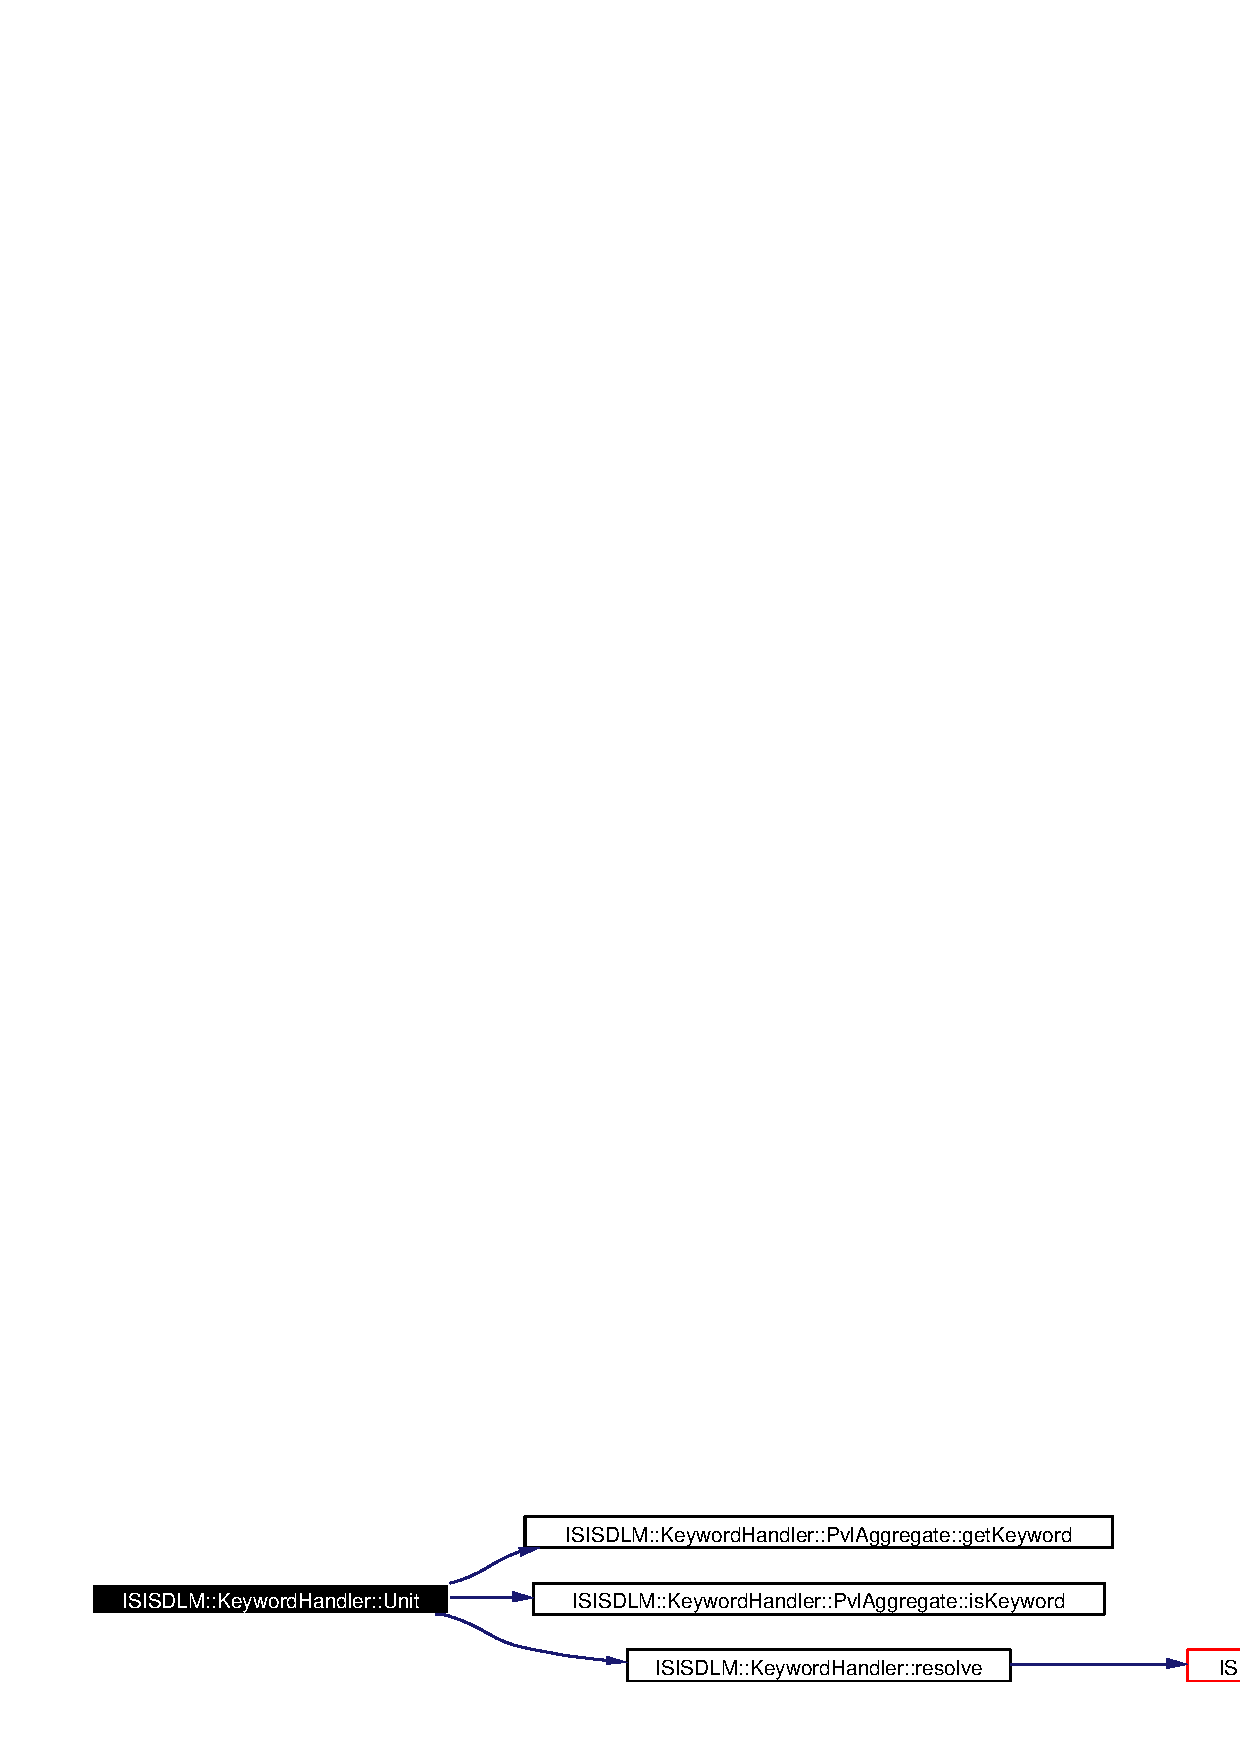
\includegraphics[width=397pt]{classISISDLM_1_1KeywordHandler_a6_cgraph}
\end{center}
\end{figure}


\subsection{Member Data Documentation}
\index{ISISDLM::KeywordHandler@{ISISDLM::Keyword\-Handler}!_kspec@{\_\-kspec}}
\index{_kspec@{\_\-kspec}!ISISDLM::KeywordHandler@{ISISDLM::Keyword\-Handler}}
\subsubsection{\setlength{\rightskip}{0pt plus 5cm}{\bf Pvl\-Spec\-List} {\bf ISISDLM::Keyword\-Handler::\_\-kspec}\hspace{0.3cm}{\tt  [private]}}\label{classISISDLM_1_1KeywordHandler_r0}


\index{ISISDLM::KeywordHandler@{ISISDLM::Keyword\-Handler}!ID@{ID}}
\index{ID@{ID}!ISISDLM::KeywordHandler@{ISISDLM::Keyword\-Handler}}
\subsubsection{\setlength{\rightskip}{0pt plus 5cm}const char $\ast$const {\bf ISISDLM::Keyword\-Handler::ID} = \char`\"{}\$Revision: 1.2 \$ \$Date: 2004/11/02 15:38:53 \$\char`\"{}\hspace{0.3cm}{\tt  [static]}}\label{classISISDLM_1_1KeywordHandler_s0}


Class version. 



The documentation for this class was generated from the following files:\begin{CompactItemize}
\item 
{\bf Keyword\-Handler.h}\item 
{\bf Keyword\-Handler.cpp}\end{CompactItemize}
